\subsection{Current Visualisation Systems}
\label{sec:current-systems}
Extremely large datasets are commonplace within radio astronomy research. 
As this research progresses, the datasets are predicted to balloon in size even more at ever faster rates.
Advances in astronomical technology, such as larger detectors, increases in bandwidth, and astrophysical simulations, drive the need for visualisation solutions.
Specialised systems have been developed to cater to this aspect of astronomy data, as well as to astronomy researchers. 
While not all of these systems attempt to apply a generalist approach to volumetric data visualisation, important points can be taken from the systems reviewed.
The system architectures and strategies employed to handle the enormous amount of data produced by modern radio astronomy data-capturing instruments emphasise points that can be applied to various systems, as there are some shared goals.
Sources~\cite{Ferrand2016, Hassan2011, Naiman2016, Kent2013, Shneiderman2008} highlight a need for a generic standalone, cross-platform application capable of processing and visualising large amounts of volumetric data. 
These visualisations, used in addition to traditional statistical visualisations, have complementary effects on knowledge extraction by communicating information clearly and effectively~\cite{Caldarola2017, Goodman2012, Naiman2016, Rosenblum1994} especially as the variety of data grows and becomes more complex.
% want for a cross platform appication capable of processing and visualising various types of astronomy data formats, especially as those format grow evermore complex

\subsubsection{Big Data Visualisation Systems}
While not specifically geared towards astronomy data visualisation, these systems face similar issues handling large amounts of scientific data, and reviewing some of these systems could add valuable insight which can be applied to the development of radio astronomy visualisation systems.

% The big data era has made many very large datasets available, they are dynamic and characterised by high variety and volitility where new data is constantly being added
\textit{Big data} as a term can be defined as ``datasets whose size is beyond the ability of software tools to capture, store, manage, and process''~\cite{manyika2011, Sneiderman1996} or ``data which exceeds the capabilities of commonly used hardware environments and software tools to capture, manage, and process it within a reasonable amount of time''~\cite{merv2011}.
These datasets have characteristics relating to the three V's of \textit{big data}: volume, velocity, and variety.
As volume increases, problems involving processing, storing, and extracting knowledge arise.
When variety increases it complicates the storage and analysis of the data because of the different structures of data being stored.
Velocity relates to the speed at which data is generated, this has the potential to compound the issues of storing and processing a high volume of data~\cite{Caldarola2017}.
This is because processing data takes time and if data is not process fast enough it creates a backlog when new data is inbound.

There are various software packages and platforms to assist the user in making sense out of massive amount of information, each tailored to a specific use case.
For big data visualisation and analytics, great consideration must be put into the method of visualisation because the structure of the data affects the resulting visualisation.
Generally the tools value flexibility and user convenience.
By making these tools available on multiple platforms for ease of access and by having them be programming language agnostic, allowing the user to cutomise their workspace.
% There is a wide range of data plotting software that can be used to tailor a solution according to the data that needs to be analysed.
% RNeo4J, Statnet, Tableau, infogram, Tulip

A general solution to visualisation and analytics is complicated because it is impossible to account for all methods of visualisation and for the variety of data.
But most are aimed towards business analytics.
Some examples of data visualisation software for specific data types are:
\begin{itemize}
  \item Timeline - specialised to create interactive timelines from a spreadsheet
  \item Commetrix and Cuttlefish - used for dynamic network visualisation and analysis
  \item Cytoscape - used for visualising molecular interaction networks and biological pathways, originally designed for biological research but is now also used for complex network visualisation and network analysis
\end{itemize}

Current systems used for exploration and visualisation cannot handle the size of many contemporary datasets and restrict themselves to analysing only comparatively small data-sets.
This is mainly due to them using a brute force method of visualising the entire dataset regardless of how it will appear on a display~\cite{Bikakis2018}.
% offline - use a single local machine to generate the visualisations

The free-to-use game engine Unity~\cite{Marchetti2020, Ferrand2016, Ferrand2018} and the open source three-dimensional modelling and animation software Blender~\cite{Taylor2015, Taylor2016, Kent2013, Naiman2016} have been used for fast prototyping of various astronomy visualisation systems.
Blender is favoured for three-dimensional rendering capabilities and it three-dimensional space manipulation tools,
particularly useful for generating animations and graphics with astronomy data.

\paragraph{ParaView}
ParaView~\cite{Ahrens2005}, is an example of a tool created for scientists to visualise and analyse extremely large data-sets,
while emphasising the workflows of the domain experts.
It highlights speed and performance as key aspects of the software's functionality.
Its rendering strategy involves executing programs in parallel on either shared or distributed memory resources.
% supports hardware accelerated parallel rendering
% acheives interactive rendering performance via level-of-detail techniques
It can achieve high frame rates suitable for interaction by utilising level-of-detail techniques.
These level-of-detail techniques, also known as progressive visualisation, involve storing the dataset at many different resolution levels, which are also know as mipmaps.
They reduce the amount of data that has to be rendered, which also impacts the quality of the visualisation.
The dataset being visualisation must find a balance between the resolution of the data and the performance of the system
%  advantage of progressivly refining a coarse model of the data
% But leveraging the advantages of refining a coarse model of data and refining parts as the user works through the data.
\begin{figure*}
    \centering
    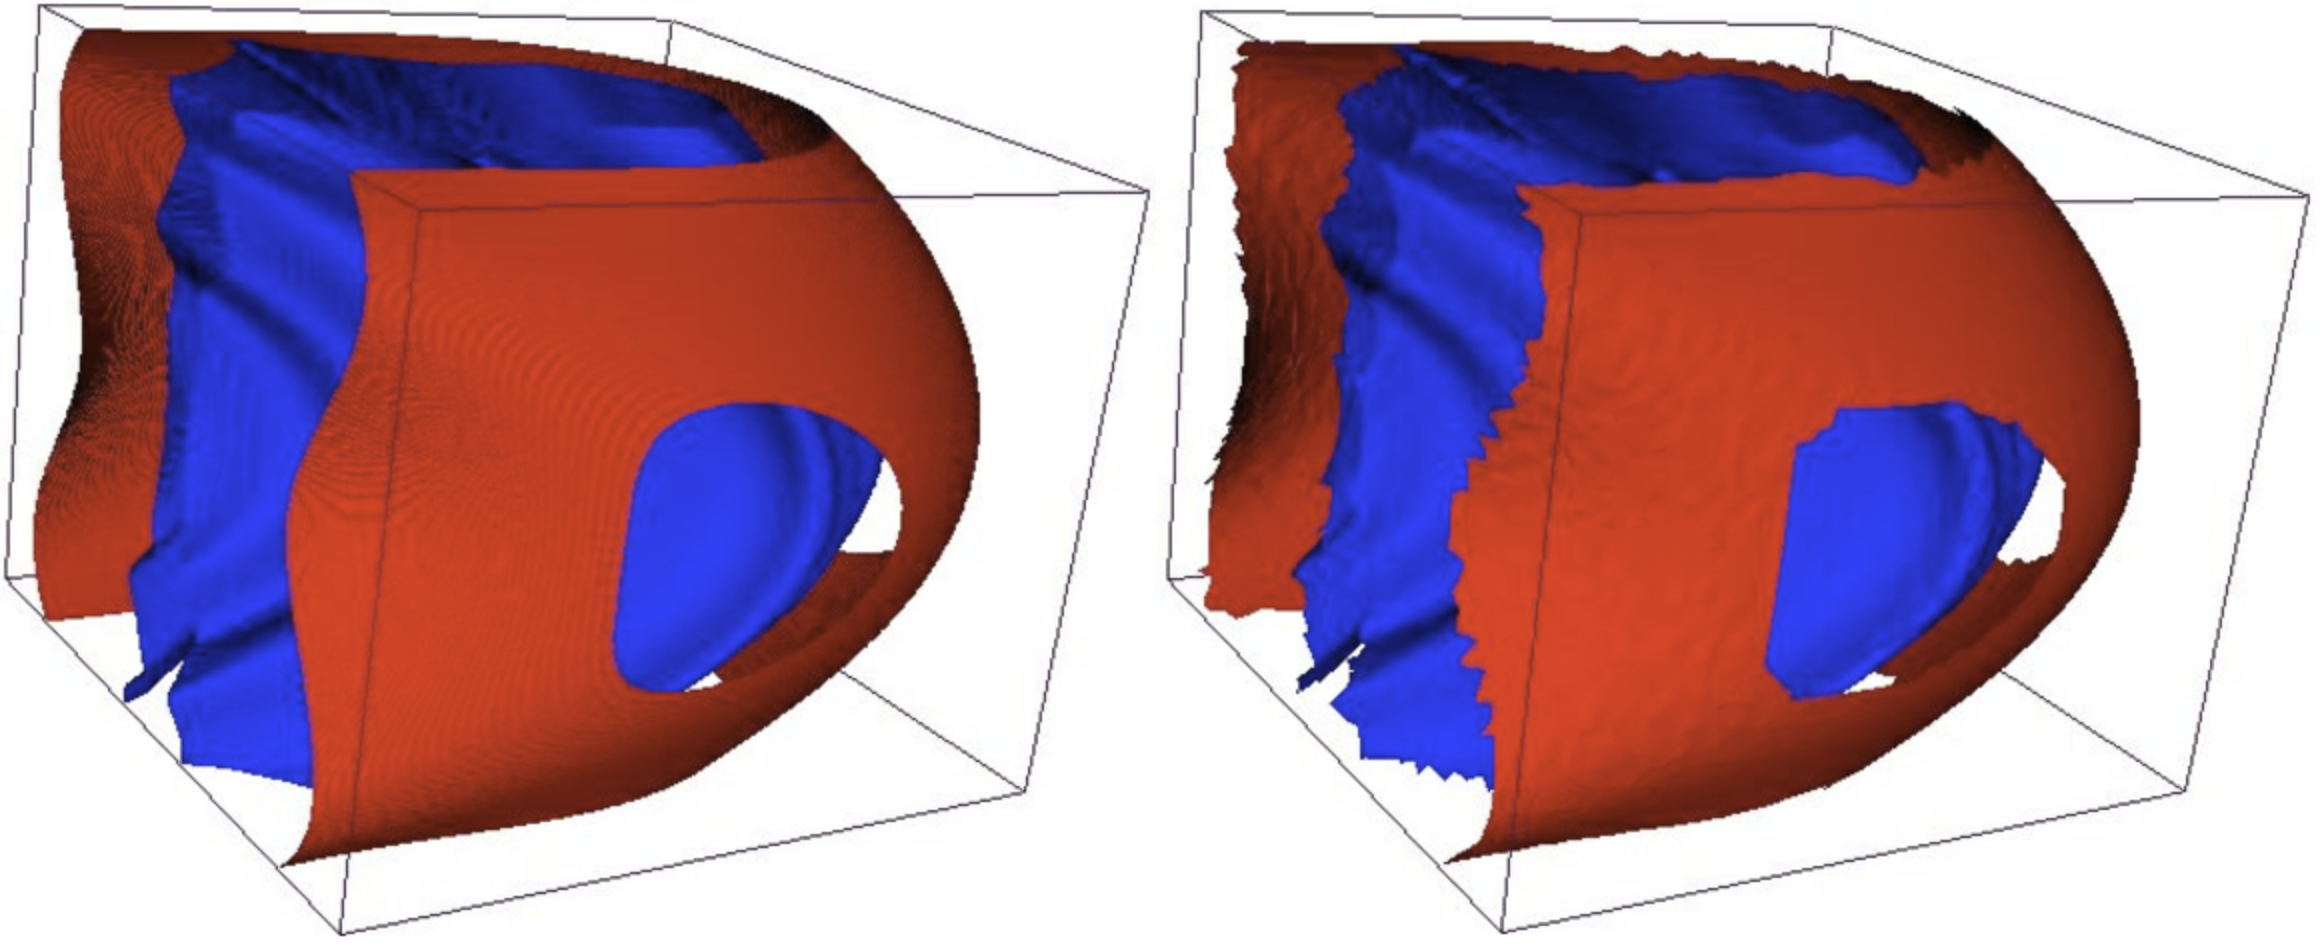
\includegraphics[width=0.6\linewidth]{figures/paraview.png}
    \caption{An example of a level-of-detail technique specified by ParaView. The model on the left is rendered at a higher resolution than the one on the right. While the quality of rendering is impacted, but improving rendering performance by having a lower resolution model to visualise.}
    \label{fig:paraview}
\end{figure*}
% multi-resolution representations or mipmaps as well as parallelism can be used to improve both visualisation and rendering performance
% describing and exploratory mode (a graphical user interface toll is used to explore the dataset) and batch mode (scripting and programming languages are used to write and execute a program

% portability - for to function on the diverse computational resources available and differnt displays (VR)
% accessability - ability to gain access to, setup, and run the tool
% extensibility - ability to easily add new functions to the tool
% describes a large dataset as data that exceeds the resource limit of a single machine
% uses a layered architecture
ParaView uses a layered architecture~\cite{Ahrens2005}.
The VTK foundation layer handles the data representation and algorithms~\cite{Ahrens2005}.
The second layer handles the parallel extensions to the visualisation toolkits, while supporting streaming of many data types and parallel execution.
The third and final layer is ParaView itself, which provides a graphical user interface and the visualisations.

\subsubsection{Astronomy Data Visualisation Systems}
Among the systems used to process and visualise \textit{big data} datasets there are some systems exclusively made for astronomy data.
% \cite{Lan2021}
% a comprensive catalogue of the current state of visualisation technologies present in astrophsyics

\paragraph{CARTA}
The acronym CARTA stands for Cube Analysis and Rendering Tool for Astronomy~\cite{Comrie2021}.
% aim is to provide a usable and scalable system utilising modern web technologies and parallel computing
Its objective is to provide a usable and scalable system using modern web technologies,
and its main hallmark is being able to load and render a dataset of several Terabytes in a matter of second.
It achieves this by storing the dataset at various levels of resolution and sending only the required requested data to produce a comprehensible rendering, instead of attempting to render the whole dataset at once.
% hosts large datasets remotely, uses the remote approach
It makes use of the client-side remote rendering approach for handling large datasets, by hosting them on a remote server.
% access the remote data from a local web-based client
A local web-based client accesses the data through a network connection, the data is transferred to the client and rendered within the web browser.
% focuses on being able to load a dataset of several TeraBytes worth of data in a matter of seconds
% designed for the ALMA, VLA, SKA pathfinders
It is designed for the ALMA, VLA, and SKA pathfinders
% works with data types such as FITS, CASA, MIRIDA, and HDF5
and works with data types commonly used in astronomy research such as FITS, CASA, MIRIAD, and HDF5.

\paragraph{i-DAVie}
This software for data cube exploration within a virtual environment, 
providing tools to navigate and interact with the visualisations.
Functionality to view metrics and interactively mask regions of data in the VR environment to catalogue sources is particularly useful.
% They enable a unique and immersive perspective on the data and allow intuitive interactions with the data
The VR environment integration enables a unique and immersive perspective of the data, affording intuitive interactions.
% created using the Unity game engine
It was created using the Unity game engine and uses the client-server architecture within its design~\cite{Marchetti2020}.
% system design uses the client-server model with server side rendering, where the visualisation is generated on the server and the frames are streamed to the front-end
It stores the datasets on the server but also renders the visualisation using the server.
% takes computational load off of the client but adds latency to the inteactions
% This approach takes computational load off the client but adds latency to the visualisation feedback as the user interactions must first be sent to the server, then visualisation is then updated based on the received interaction, and finally the frames are sent back to the client.
% The latency is proportional to the distance the client is from the server, and therefore latency increases as the distance between the client and server increases.
%   interactions performed on the client is sent to the server
%   visualisation is udated based on the input
%   frames are sent back to the client
A prototype system similar to i-Davie created for public outreach~\cite{Ferrand2018}, is a tethered standalone system which means that the server and the client are connected to each other with a physical connector such as a cable.
It also uses Unity with custom scripts to visualise FITS files and displays the visualisation in a VR environment using the HTC Vive. 
It can produce iso-surface or volumetric visualisations of a dataset.

\paragraph{Frelled}
A general-purpose astronomy viewer~\cite{Taylor2015} which uses a set of Python scripts to create three-dimensional visualisations of FITS files inside Blender, and is used for visual source extraction, cataloguing, and analysis.
It can visualise large datasets of roughly 600,000 points at more than 10 frames per second, while providing tools to mask data interactively, functionality similar to i-DAVie.
The FITS file can be explored in a three-dimensional space, instead of two-dimensional slices.
It provides a significant speedup in source cataloguing compared to other viewers, facilitating the recording of hundreds of sources a day.
Visual source extraction by an astronomer is still currently more effective than automated processes.
% motivations
%   desire to view 3D datasets in a 3D space
%   the need to rapidly mask regions of the data

\paragraph{AstroBlend}
A Python package for Blender~\cite{Naiman2016}, combining the three-dimensional capabilities of Blender with astronomy analysis tools.
Allows astronomers to analyse data alongside visualisations, while simplifying the importing process.
% simplifies the importing process of importing astrophysical datasets, generating visualisations, and anyalysis plots

\paragraph{SlicerAstro} % other good sources
A multi-platform open-source package for visualising and processing medical images,
which is an extension of the open-source software 3D slicer~\cite{Fedorov2012}.
It aim is to provide an interactive three-dimensional visual analytics tool using two-dimensional displays and interaction devices.
It is implemented using C++.
Its features include interactive filtering, three-dimensional masking and modelling, and support for FITS files.

\paragraph{E0102-VR}
\cite{Baracaglia2019}
An experimental standalone application using a VR display and interaction devices.
Its aim is to demonstrate the benefits of using human depth perception for fast and accurate characterisation of three-dimensional structures.
It explores the scientific potential of VR for displaying multi-dimensional datasets in astronomy and astrophysics.
The system pre-processes datasets into an iso-surface representation as it does not currently support volume rendering.
These pre-processed datasets can be swapped out with no effect on the functionality, but the system is currently coupled to a single dataset (SNR E0102) for experimental purposes.
The size of the dataset is limited because all the computation is done on a single computer.
% the pre-compiled/pre-processed dataset can be swapped out with no major loss of functionality
%   currently coupled to a single dataset (SNR E0102) for experimentation purposes
% uses isosurfaces to represent the visualisation
% limits the size of the datasets that can be used as all computation is done on a single computer